\cleardoublepage
\phantomsection
\addcontentsline{toc}{chapter}{Introduction}
\chapter*{Introduction}
\lhead{\textit{Introduction}}
\setlength{\headheight}{14pt}

\begingroup
\setcounter{section}{0} 
\renewcommand{\thesection}{\arabic{section}.} 

\section{Context and Motivation} \label{contextMotivation}
Over the past decade, blockchain technology has evolved from a fringe experiment to a multi-billion-dollar industry.  
Yet security has not kept the same pace: in calendar year 2024 alone, \textit{more than \$2 billion in value were irreversibly lost because of smart‑contract hacks and protocol exploits, with DeFi\footnote{DeFi (Decentralized Finance) refers to financial services built on blockchain networks, eliminating intermediaries through smart contracts.} as the primary target of crypto hacks}. In the picture \ref{fig:stolen-funds}, from a report of Chainalysis \cite{chainalysisblog}, you can observe the rising trend of stolen funds and hacks in decentralized ecosystems.

\begin{figure}[h]
    \centering
    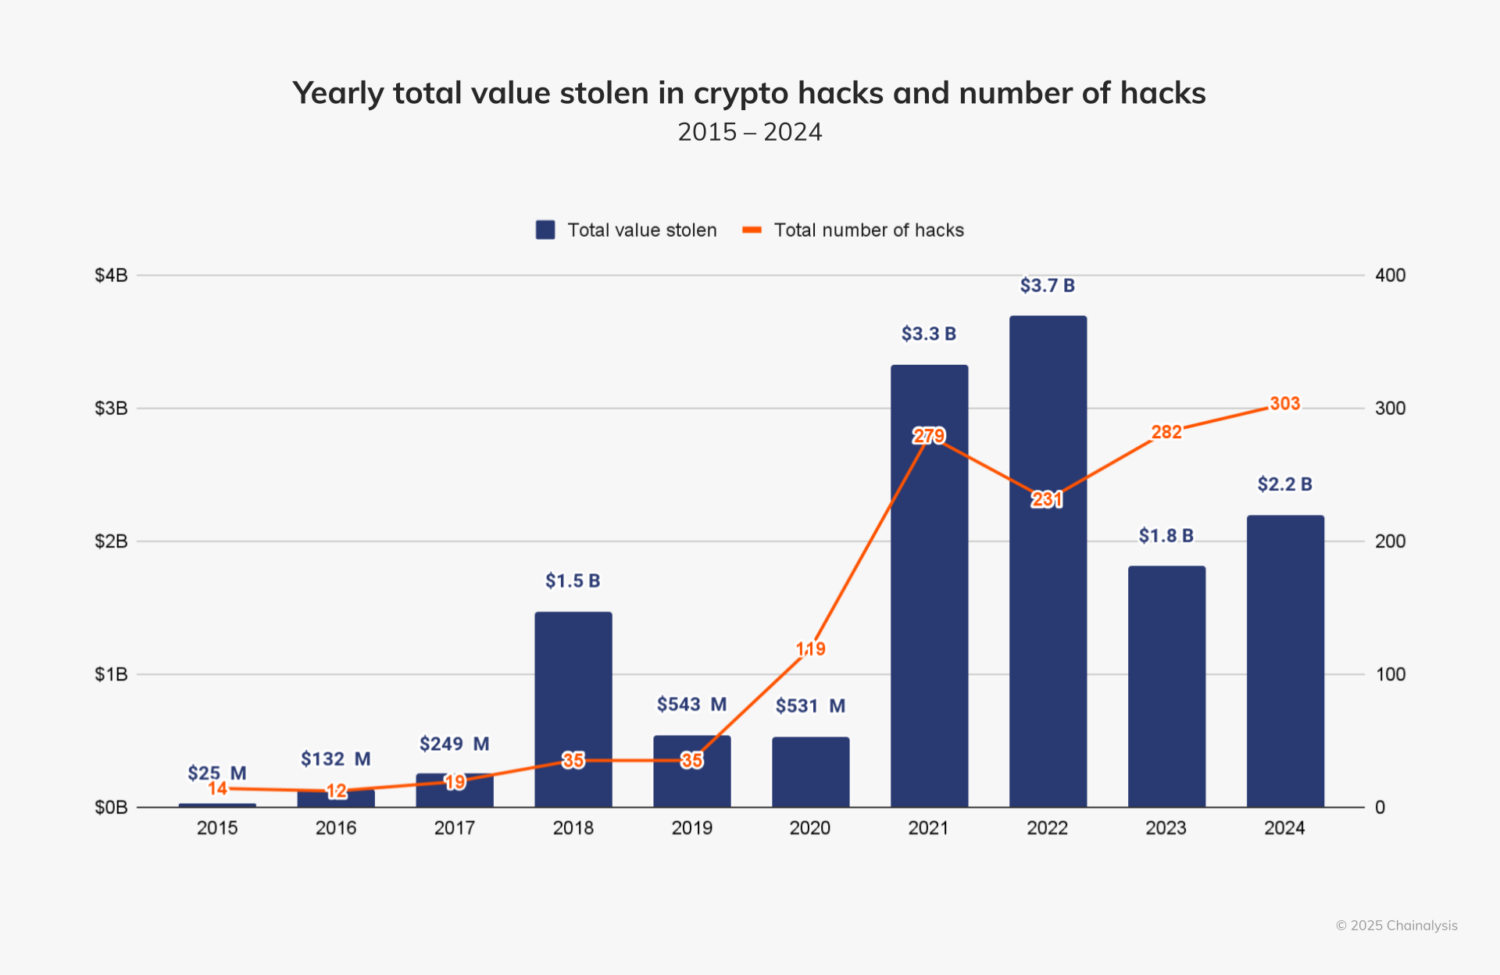
\includegraphics[width=1.0\linewidth]{Images/Introduction/stolen-funds-chainanalysis.png}
    \caption{Yearly total value stolen in crypto hacks and number of hacks from 2015 to 2024.}
    \label{fig:stolen-funds}
\end{figure}

Attackers enjoy asymmetric advantages; they can remain anonymous, watch code evolve in public, and strike at the most opportune moment. At the same time, honest security researchers must reveal an exploit to prove its existence and then hope that a project honors its bounty commitment.
Traditional bug‑bounty workflows, therefore, introduce two fundamental frictions:

\begin{enumerate}
    \item \textbf{Trust asymmetry}: the researcher must fully disclose the exploit before payment is guaranteed, risking front‑running or litigation if the vulnerability is down‑played.
    \item \textbf{Operational overhead}: Projects drown in low‑quality or spam reports and often need third‑party escrow services to arbitrate payments.
\end{enumerate}

\noindent
\textbf{Zero‑Knowledge Proofs of Exploit (zkpoex)} break this deadlock.  
By committing to a formal specification of \textit{correct} state transitions and then proving, in zero‑knowledge, that a private input violates at least one of those invariants, a white‑hat hacker can demonstrate the presence of a flaw without disclosing the exploit itself.  
The open‑source framework \textit{zkpoex}\cite{zkpoex} extends this paradigm, combining a RISC‑V‑based\footnote{RISC-V is an open-source, modular, and royalty-free instruction set architecture (ISA) designed to be simple, extensible, and suitable for everything from microcontrollers to supercomputers.}
 zkVM\footnote{zkVM (Zero-Knowledge Virtual Machine) is a virtual machine that executes computations while generating zero-knowledge proofs of their correctness. This enables trustless verification of program execution, a key concept in blockchain scalability and privacy. A detailed discussion follows in Section \ref{zkvm}. } with an Ethereum interpreter so that any Solidity contract can be audited in a wholly trustless setting.
The vision is compelling: automatic bounty pay‑outs, instant verifiability, and no leak of exploit details, exactly the properties that classical disclosure channels lack.

\section{Problem Statement}\label{sec:core-problem}
Blockchain security today suffers from a paradox: vulnerabilities are straightforward to exploit yet notoriously hard to disclose safely. Smart-contract authors need cryptographic assurance that a reported flaw is genuine before acting, while ethical hackers need economic assurance that disclosure will be rewarded rather than front-run.  Bridging this chasm demands a protocol able to transform the \textit{existence} of an exploit into a \textit{verifiable} mathematical statement, one that can be checked on-chain without revealing the exploit itself. The remainder of this section formalises that challenge and breaks down the system requirements that drive \textit{zkpoex} design.

\subsection*{From “exploitable’’ to “provably exploitable’’}
Smart-contract audits ultimately ask a binary question:  

\begin{quote}
    \centering
    \textbf{Does there exist a calldata~$c$ that induces an \textbf{invalid state transition} in the contract’s execution?}
\end{quote}

Finding such an input is only half the battle; \textit{convincing the contract owner without revealing it} is the harder half.  
This dilemma crystallizes into three interlocking technical challenges:

\begin{enumerate}[label=\textbf{C\arabic*}:, leftmargin=1.8cm]
    \item \textbf{Specification Gap}: Real-world contracts rarely come with a
    executable \textit{specification}. Without formal post-conditions (e.g.\ invariants on balances, total supply, access-control flags), a proof system has nothing to assert against.
    \vspace{2pt}
    \item \textbf{Zero-Knowledge Execution}: Even with a clear specification in hand, we still have to replay the contract call inside a zero-knowledge proving system without exposing any data. Building a huge custom circuit that hard-codes every single EVM instruction would be far too slow and complex. A better approach is to use a general-purpose zero-knowledge virtual machine (zkVM) and run an ordinary EVM interpreter inside it; this keeps the proof trace compact and manageable for everyday transactions.
    \vspace{2pt}
    \item \textbf{Trustless Settlement}: Once a proof is generated, payment must be \textit{automatic}. Any off-chain escrow would reintroduce trust and timing risk, so the verification logic must live on-chain, remain gas-efficient, and emit side effects (bounty payout, pausing the contract, and related actions) atomically.
\end{enumerate}

\subsection*{Why existing approaches fall short}

Prior art demonstrates zero-knowledge proofs of exploitability for firmware\cite{green2023efficient} and LLVM\footnote{LLVM (Low Level Virtual Machine) is a compiler infrastructure that produces binaries and intermediate code representations used for optimization and cross-platform compilation across various programming languages.}binaries\cite{cuellar2023cheesecloth} (the papers are detailed in Section \ref{slr} of the Introduction Chapter); however, none address the peculiarity of smart contracts. To the best of our knowledge, this thesis provides the first scientific and academic documentation of zero-knowledge proofs of exploitability in the context of smart contract security. Below, we outline two fundamental challenges that distinguish the smart contract setting from previous works: 

\begin{itemize}
    \item \textbf{State Explosion}:  Unlike ordinary programs, a smart contract’s execution depends on persistent, on-chain state (e.g., user balances, contract storage). This state is stored in a Merkle-Patricia trie, a cryptographic data structure that allows efficient verification of key-value pairs. To prove an exploit, the prover must reproduce just the slice of the global state that the transaction touches, otherwise, the proof grows enormous. Hence the term \textit{state explosion} \cite{StateExplosion}.
    \item \textbf{Trustless Finality}: On-chain attacks finish in a single block, so the fix (paying the bounty and optionally pausing the contract) must also complete in one atomic transaction. Any scheme that needs off-chain arbitration reintroduces the very trust issues we are trying to remove.
\end{itemize}

\subsection*{Formalisation of the Problem}

Formally, let:

        \begin{equation*}
          \mathcal{M} : \bigl(s,\,c\bigr)\;\mapsto\; s' 
        \end{equation*}
        
be the EVM transition function that maps an initial state~$s$ and calldata~$c$ to a new state~$s'$. Let~$\Phi(s,s')$ denote a decidable predicate capturing all contractual invariants. The \textit{zkpoex} problem is to design a protocol where a prover convinces a verifier of the statement

    \[
      \exists\,c \;.\; \lnot\Phi\bigl(s,\mathcal{M}(s,c)\bigr)
    \]

\textit{without revealing~$c$} and such that the following properties hold:

\begin{enumerate}[label=\textit{(\alph*)}]
    \item \textbf{Soundness}: No adversary can convince an honest verifier unless a real exploit exists.
    \item \textbf{Zero-Knowledge}: The verifier learns nothing about~$c$ beyond the fact that an exploit exists.
    \item \textbf{Atomicity}: Upon acceptance, the bounty is disbursed within the same Ethereum transaction that verifies the proof.

\end{enumerate}

The formula says:

\begin{quote}
    “There exists a calldata $c$ such that executing $c$ from the current blockchain state $s$ produces a successor state $s'$ where the \textbf{state transition} $(s \!\to\! s')$ violates at least one contract rule $\Phi$.”
\end{quote}

Solving the problem above removes the fundamental trust bottleneck that plagues traditional vulnerability disclosure and lays the groundwork for \textit{specification-driven} smart-contract development, where proving a bug becomes as routine as running unit tests.

\section{Research Objectives}
Although individual research papers have demonstrated proofs‑of‑concept(PoC) for \textit{software} binaries, the literature lacks a system that is \textit{tailor‑made for blockchain} and that leverages modern, transparent proof systems.  
Consequently, this thesis pursues four concrete objectives:

\begin{enumerate}
    \item \textbf{Design} a protocol that allows a prover to convince a verifier that a smart‑contract exploit exists \textit{without} revealing calldata, bytecode patches, or private keys.
    \item \textbf{Implement} an end‑to‑end prototype: \texttt{zkpoex v0.1.0}, built on \texttt{Risc0}\cite{risc0} and \texttt{Rust‑EVM}\cite{rustEVM}, capable of handling realistic scenarios.
    \item \textbf{Evaluate} the performance, scalability and security assumptions of \texttt{zkpoex v0.1.0} through extensive benchmarking and profiling (e.g.\ proving time, proof size or cycle counts), \textit{without} direct comparison to external toolchains.
    \item \textbf{Validate} the protocol with real‑world case studies on public Ethereum testnets, reporting empirical results proving time, on‑chain verification gas, and bounty‑payout latency, to substantiate the effectiveness of the proposed approach, again \textit{without} cross‑tool‑chain benchmarks.

\end{enumerate}


\section{Research Methodology}\label{slr} %DA SPOSTARE a 2.1

A \texttt{Systematic Literature Review (SLR)} was carried out to chart current research on Zero‑Knowledge Proofs of Exploitability (or Exploit).  
The review was organised following Kitchenham’s three‑stage process \cite{Kitchenham}:

\begin{enumerate}[label=\texttt{(\roman*)}]
    \item \textbf{Planning}: Research questions were refined and trial search strings evaluated.  
          An illustrative query was:
\begin{verbatim}
("vulnerability disclosure" OR "vulnerabilities disclosure")
AND blockchain AND ("ZKPs" OR "Zero Knowledge Proofs"
OR "ZKP") -"IoT" -"machine learning"
\end{verbatim}

    \item \textbf{Conducting}: The engines \textit{IEEE Xplore}, \textit{ACM Digital Library}, \textit{arXiv}, and \textit{Google Scholar} were searched for publications dated 2013–2025.

    \item \textbf{Reporting}: Automatic filters were first applied, then a manual screening followed.  
          Titles and abstracts were checked against \textit{inclusion} criteria (blockchain relevance, demonstrable exploit, peer‑review, English language) and \textit{exclusion} criteria (IoT or ML focus, topics unrelated to vulnerability disclosure, grey literature lacking technical substance).  
          Surviving papers underwent full‑text review; quality was logged on a five‑point Likert scale covering rigour, reproducibility and relevance.  
           The process yielded \textbf{two} peer-reviewed primary studies; an additional survey paper and an open-source prototype were retained as complementary evidence that sharpens the problem framing but do not themselves constitute peer-reviewed solutions.
\end{enumerate}

\vspace{1em}
\noindent\textbf{Primary studies}

\begin{enumerate}[label=\arabic*.]

    \item \textbf{Hardware-oriented proof generation: \textit{Efficient Proofs of Software Exploitability for Real-world Processors} \cite{green2023efficient}}\label{sec:green}

          The study targets the MSP430, a 16-bit microcontroller family often embedded in low-power devices such as smart meters and sensor nodes.  
          The authors model the entire instruction set in \textit{Verilog}, a hardware-description language that can be compiled into an arithmetic circuit suitable for a zk-SNARK back-end.  
          zk-SNARKs (Zero-Knowledge Succinct Non-Interactive Arguments of Knowledge, which will be introduced together with the basis of ZKPs and related history in Section \ref{zkpChap}), briefly, allow a prover to convince a verifier that a computation was executed correctly without revealing intermediate data, while keeping both proof size and verification time small.  
          By reducing gate count and re-ordering constraints, the paper shows that one can generate a proof of exploitability whose cost is linear in the execution trace, rather than logarithmic.  
          In practical terms, this means that an attacker could demonstrate control-flow hijacking on a firmware image without disclosing the payload, and the vendor could check the proof in milliseconds.  
          The work, therefore, supplies a concrete example of how verifiable proofs-of-exploit can enable fair disclosure in resource-constrained environments.

    \item \textbf{Compiler-driven circuit synthesis: \textit{Cheesecloth: Zero Knowledge Proofs of Real-World Vulnerabilities} \cite{cuellar2023cheesecloth}}\label{sec:cheesecloth}

          Cheesecloth starts from LLVM Intermediate Representation (LLVM IR), the language-agnostic bytecode to which modern compilers lower C, C++, Rust, and other high-level languages.  
          It then maps LLVM IR into \textit{MicroRAM} constraints, a simplified random-access machine model widely adopted by zk toolchains, so that memory accesses become explicit Boolean conditions.  
          The framework encodes classic memory-safety properties such as buffer bounds and use-after-free checks, and it proves violations inside libswanky’s Mac-n-Cheese\cite{swanky} prover without exposing the exploit inputs.  
          From a broader standpoint, the paper illustrates how compiler infrastructure can bridge the gap between rich source languages and the restricted algebraic models accepted by zero-knowledge proof systems.  
          The strategy of compiling a real execution trace into a minimalist RAM abstraction is directly relevant to smart-contract settings, where EVM bytecode can be lifted to a RISC-V or MicroRAM dialect before proof generation.

\end{enumerate}


\subsection*{Complementary evidence}

\begin{itemize}
    \item \textbf{Applicability survey: \textit{Do You Need Zero-Knowledge Proofs?} \cite{ernstberger2024you}}\label{sec:needzk}\\
          This IACR ePrint (2024/050) offers a decision framework for privacy technologies.  
          Section 4.3, “Proving Software Exploits”, highlights the same disclosure dilemma tackled here and cites the \textit{ZkPoEX}\cite{zkpoex-old} repository as the only public attempt at a zero-knowledge exploit proof in the blockchain ecosystem.

    \item \textbf{Open-source prototype: \textit{ZkPoEX} (ETH Denver 2023) \cite{zkpoex-old}}\label{sec:zkpoex-old}\\
          Though not peer-reviewed, \textit{ZkPoEX} wraps an unmodified EVM interpreter inside RISC Zero and emits a recursive STARK attesting to an invariant failure while hiding calldata and keys.  
          Its architecture inspired the prototype in this thesis; however, obsolete dependencies and an outdated Rust toolchain required a complete re-implementation.  
          Two lessons stand out: 
          \begin{enumerate}[label=\texttt{(\roman*)}]
              \item General-purpose \textit{zkVMs} can execute contract bytecode unaltered, obviating bespoke circuits.
              \item On-chain verification removes the need for an external escrow in bounty negotiations.
          \end{enumerate}
    \item \textbf{Bug Bounty Trilemma: Beyond the Bug Bounty Programs Trilemma: Bounty 3.0’s Blockchain-ZKP Approach \cite{BugBountyPaper}}\\
          Although it proposes no exploit-proof system, the paper articulates the trust asymmetry between finder and vendor.  
          It envisages a token-incentivised, zk-enabled escrow where blockchain immutability records disclosure events and zero-knowledge proofs safeguard payload secrecy.  
          The design rationale directly mirrors the problem solved by our prototype.
\end{itemize}

Collectively, the two peer-reviewed studies supply technical foundations, while the survey, the prototype, and the Bug Bounty 3.0 paper sharpen the application context, confirming both the relevance of our research questions and the novelty of pursuing zero-knowledge exploit proofs for smart contracts.


\section{Document Structure}
The remainder of the dissertation is organised as follows:

\begin{itemize}
    \item \textbf{Chapter 1: Background and State of the Art}\\
          Surveys the architecture of blockchain systems, the structure of Ethereum transactions and smart contracts, and the theoretical underpinnings of zero-knowledge proofs and zkVMs.
    \item \textbf{Chapter 2: Proposed System Architecture}\\
          Describes the end‑to‑end design of the \texttt{zkpoex} framework: integration of the RISC0 zkVM, interoperability layers with the \texttt{Rust EVM}, and the exploit execution flow leading to proof generation.
    \item \textbf{Chapter 3: Implementation and Validation}\\
          Details the development environment (Rust + Risc0, and related tooling), the \textit{VerifierContract} deployed on Ethereum Holesky, and analytical case studies covering common smart-contract vulnerabilities such as reentrancy attack.
    \item \textbf{Chapter 4: Performance Evaluation and Results}\\
          Benchmarks \texttt{zkpoex} on representative exploits, summarising guest time, cycle counts, on-chain gas cost, and flame graph metrics for each case study.
    \item \textbf{Chapter 5: Conclusions and Future Perspectives} \\
          Reflects on the outcomes of the research, highlighting the main contributions of the \texttt{zkpoex} framework to smart-contract security; discusses the system’s current limitations, evaluates its applicability in real-world disclosure scenarios, and presents potential directions for future work.
\end{itemize}

This logical progression: \textit{problem $\rightarrow$ theory $\rightarrow$ architecture $\rightarrow$ empirical validation}, ensures that each chapter builds on the foundations laid by the previous one, guiding the reader from high‑level motivation to concrete, experimentally verified results.

\endgroup
% End local group
